\section{AES}

	\begin{frame}
		\begin{center}
			\LARGE{\textcolor{blue}{La sicurezza non basta mai: Advanced Encryption Standard}}
		\end{center}
	\end{frame}

	\subsection{AES}
	
		\begin{frame}
			\frametitle{AES}	
			\begin{itemize}
				\item AES è stato standardizzato dal NIST nel \tblue{2001} in previsione di sostituire 3DES
				\item Implementa un algoritmo \tblue{Rijndael}
				\item Usa blocchi \tblue{128 bits}
				\item Lunghezza della chiave 128, 192 o 256 bits (in genere \tblue{128})
			\end{itemize}
		\end{frame}
	
		\begin{frame}
			\frametitle{Funzionamento}
			\begin{columns}
				\begin{column}{0.45\textwidth}
					\begin{center}
						\begin{figure}
							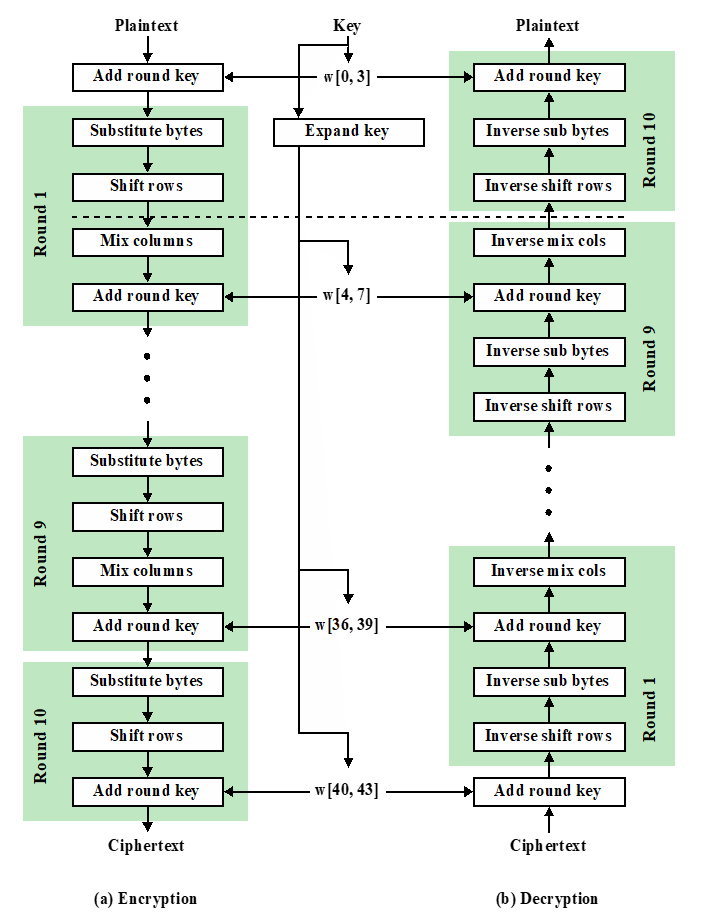
\includegraphics[width=\columnwidth]{img/aes}
							\caption{Algoritmo AES}
						\end{figure}
					\end{center}
				\end{column}
				\begin{column}{0.6\textwidth}
					\begin{itemize}
						\item Il blocco in input viene rappresentato come una matrice quadrata di bytes (4x4) chiamata \tblue{stato}
						\item Anche la chiave viene rappresentata come una matrice quadrata di bytes
						\item Il \tblue{gestore delle chiavi} ricava dalla chiave un array di 44 words da 4 byte che verranno usate come sotto-chiavi
						\item L'algoritmo si divide poi in \tblue{10 round caratterizzati} (tranne l'ultimo) da 4 fasi
					\end{itemize}
				\end{column}
			\end{columns}
		\end{frame}
	
	\subsection{Specifiche}
	
		\begin{frame}
			\frametitle{Sostituzione}
			\begin{columns}
				\begin{column}{0.45\textwidth}
					\begin{center}
						\begin{figure}
							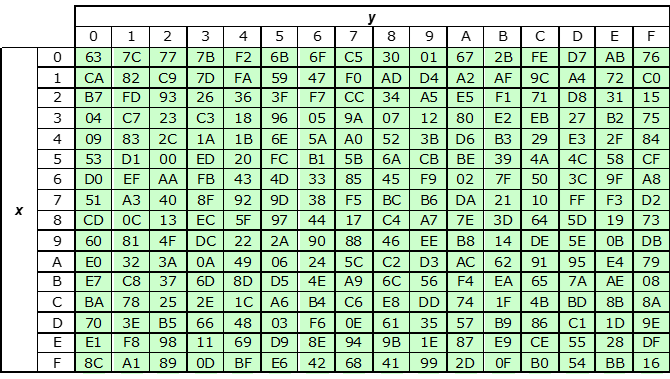
\includegraphics[width=0.8\columnwidth]{img/aesbox}
							\caption{AES S-Box}
						\end{figure}
						\begin{figure}
							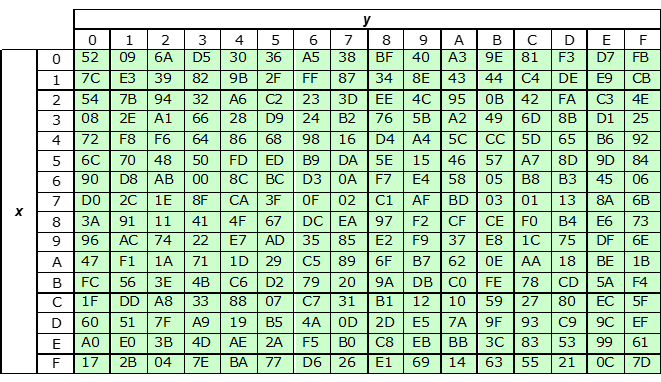
\includegraphics[width=0.8\columnwidth]{img/aesbox2}
							\caption{AES S-Box inversa}
						\end{figure}
					\end{center}
				\end{column}
				\begin{column}{0.7\textwidth}
					\begin{itemize}
						\item Sostituzione \tblue{byte per byte} attraverso la S-Box
						\item La S-Box usata è nota ed ha ottime proprietà di \tblue{non linearità}
						\item La S-Box è stata studiata a lungo per evitare che abbia \tblue{punti fissi} o \tblue{punti opposti}
					\end{itemize}
				\end{column}
			\end{columns}
		\end{frame}
	
		\begin{frame}
			\frametitle{Scostamento}
			\begin{center}
				\begin{figure}
					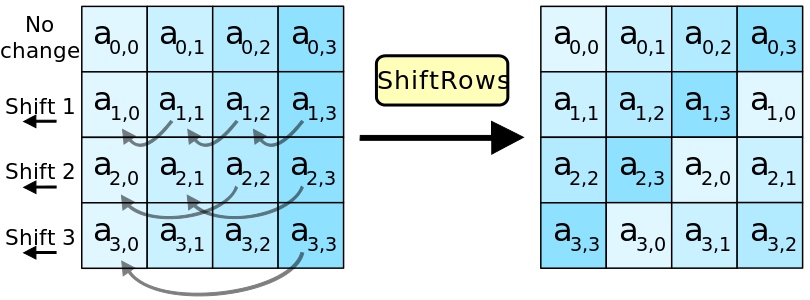
\includegraphics[scale=0.3]{img/shiftrow}
					\caption{Shift rows}
				\end{figure}
			\end{center}
			\begin{itemize}
				\item Scostamento delle righe \tblue{dipendente} dal numero di riga 
				\item L'ultima colonna diventa la \tblue{diagonale} della nuova matrice
			\end{itemize}
		\end{frame}
	
		\begin{frame}
			\frametitle{Mix columns}
			\begin{center}
				\begin{figure}
					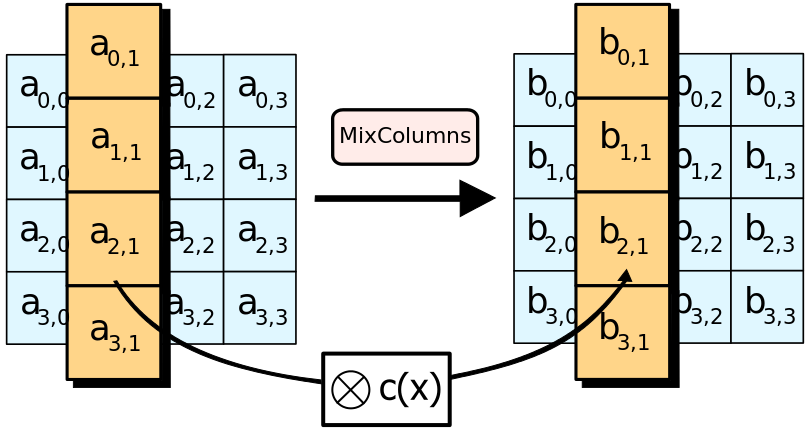
\includegraphics[scale=0.2]{img/mixcolumns}
					\caption{Mix columns}
				\end{figure}
			\end{center}
			\begin{itemize}
				\item Combinazione lineare \tblue{invertibile} delle colonne in funzione di tutti i 4 bytes di ogni colonna
				\item Insieme allo shift row applicano il criterio di \tblue{diffusione} e \tblue{confusione}
			\end{itemize}
		\end{frame}
	
		\begin{frame}
			\frametitle{Add round key}
			\begin{center}
				\begin{figure}
					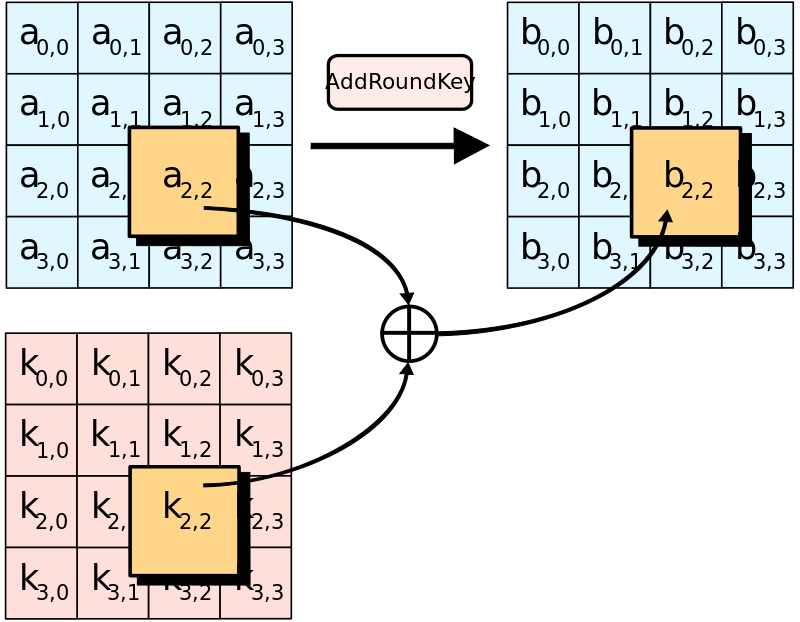
\includegraphics[scale=0.1]{img/addroundkey}
					\caption{Add round key}
				\end{figure}
			\end{center}
			\begin{itemize}
				\item \tblue{XOR} bit a bit dello stato attuale con la chiave di round
			\end{itemize}
		\end{frame}
	
		\begin{frame}
			\frametitle{Sicurezza}
			{
			\fontsize{10}{0}
			\begin{itemize}
				\item Semplice da implementare e richiede \tblue{poche risorse} (ottimo per le smart-card)
				\item NSA utilizza chiavi di 128 bits per crittografare documenti classificati \tblue{SECRET} e di 192 o 256 per i \tblue{TOP SECRET}
				\item \tblue{Distributed.net} ha effettuato il miglior attacco di forza bruta conosciuto su chiave da 64 bit impiegando circa 5 anni utilizzando potenza computazionale di volontari sparsi per il mondo
				\item Approfondita descrizione \tblue{matematica} riguardante AES solleva le maggiori preoccupazioni
				\item Nel 2002 l'attacco teorico \tblue{XSL} basato appunto su alcune proprietà matematiche ha mostrato un punto debole di AES. Computazionalmente non è applicabile.
			\end{itemize}
			}
		\end{frame}


